\section{Основная часть}
\subsection{Экспериментальное оборудование. Схема экспериментальной установки}
\subsubsection{Криостат растворения}

Экспериментальная работа проводилась со сверхпроводящими квантовыми схемами, что подразумевает оперирование системой в условиях сверхнизких температур. Во-первых это даёт возможность обеспечить переход в сверхпроводящее состояние, во-вторых, и что более важно, в этом случае равновесная заселённость близка к чистому состоянию $|0\rangle$. Криостат растворения Oxford Instruments Triton DR-200, изображённый на Рисунке 16, стабильно обеспечивает температуру порядка 20 мК. 

\begin{figure}[h]
	\begin{minipage}[h]{0.49\linewidth}
		\center{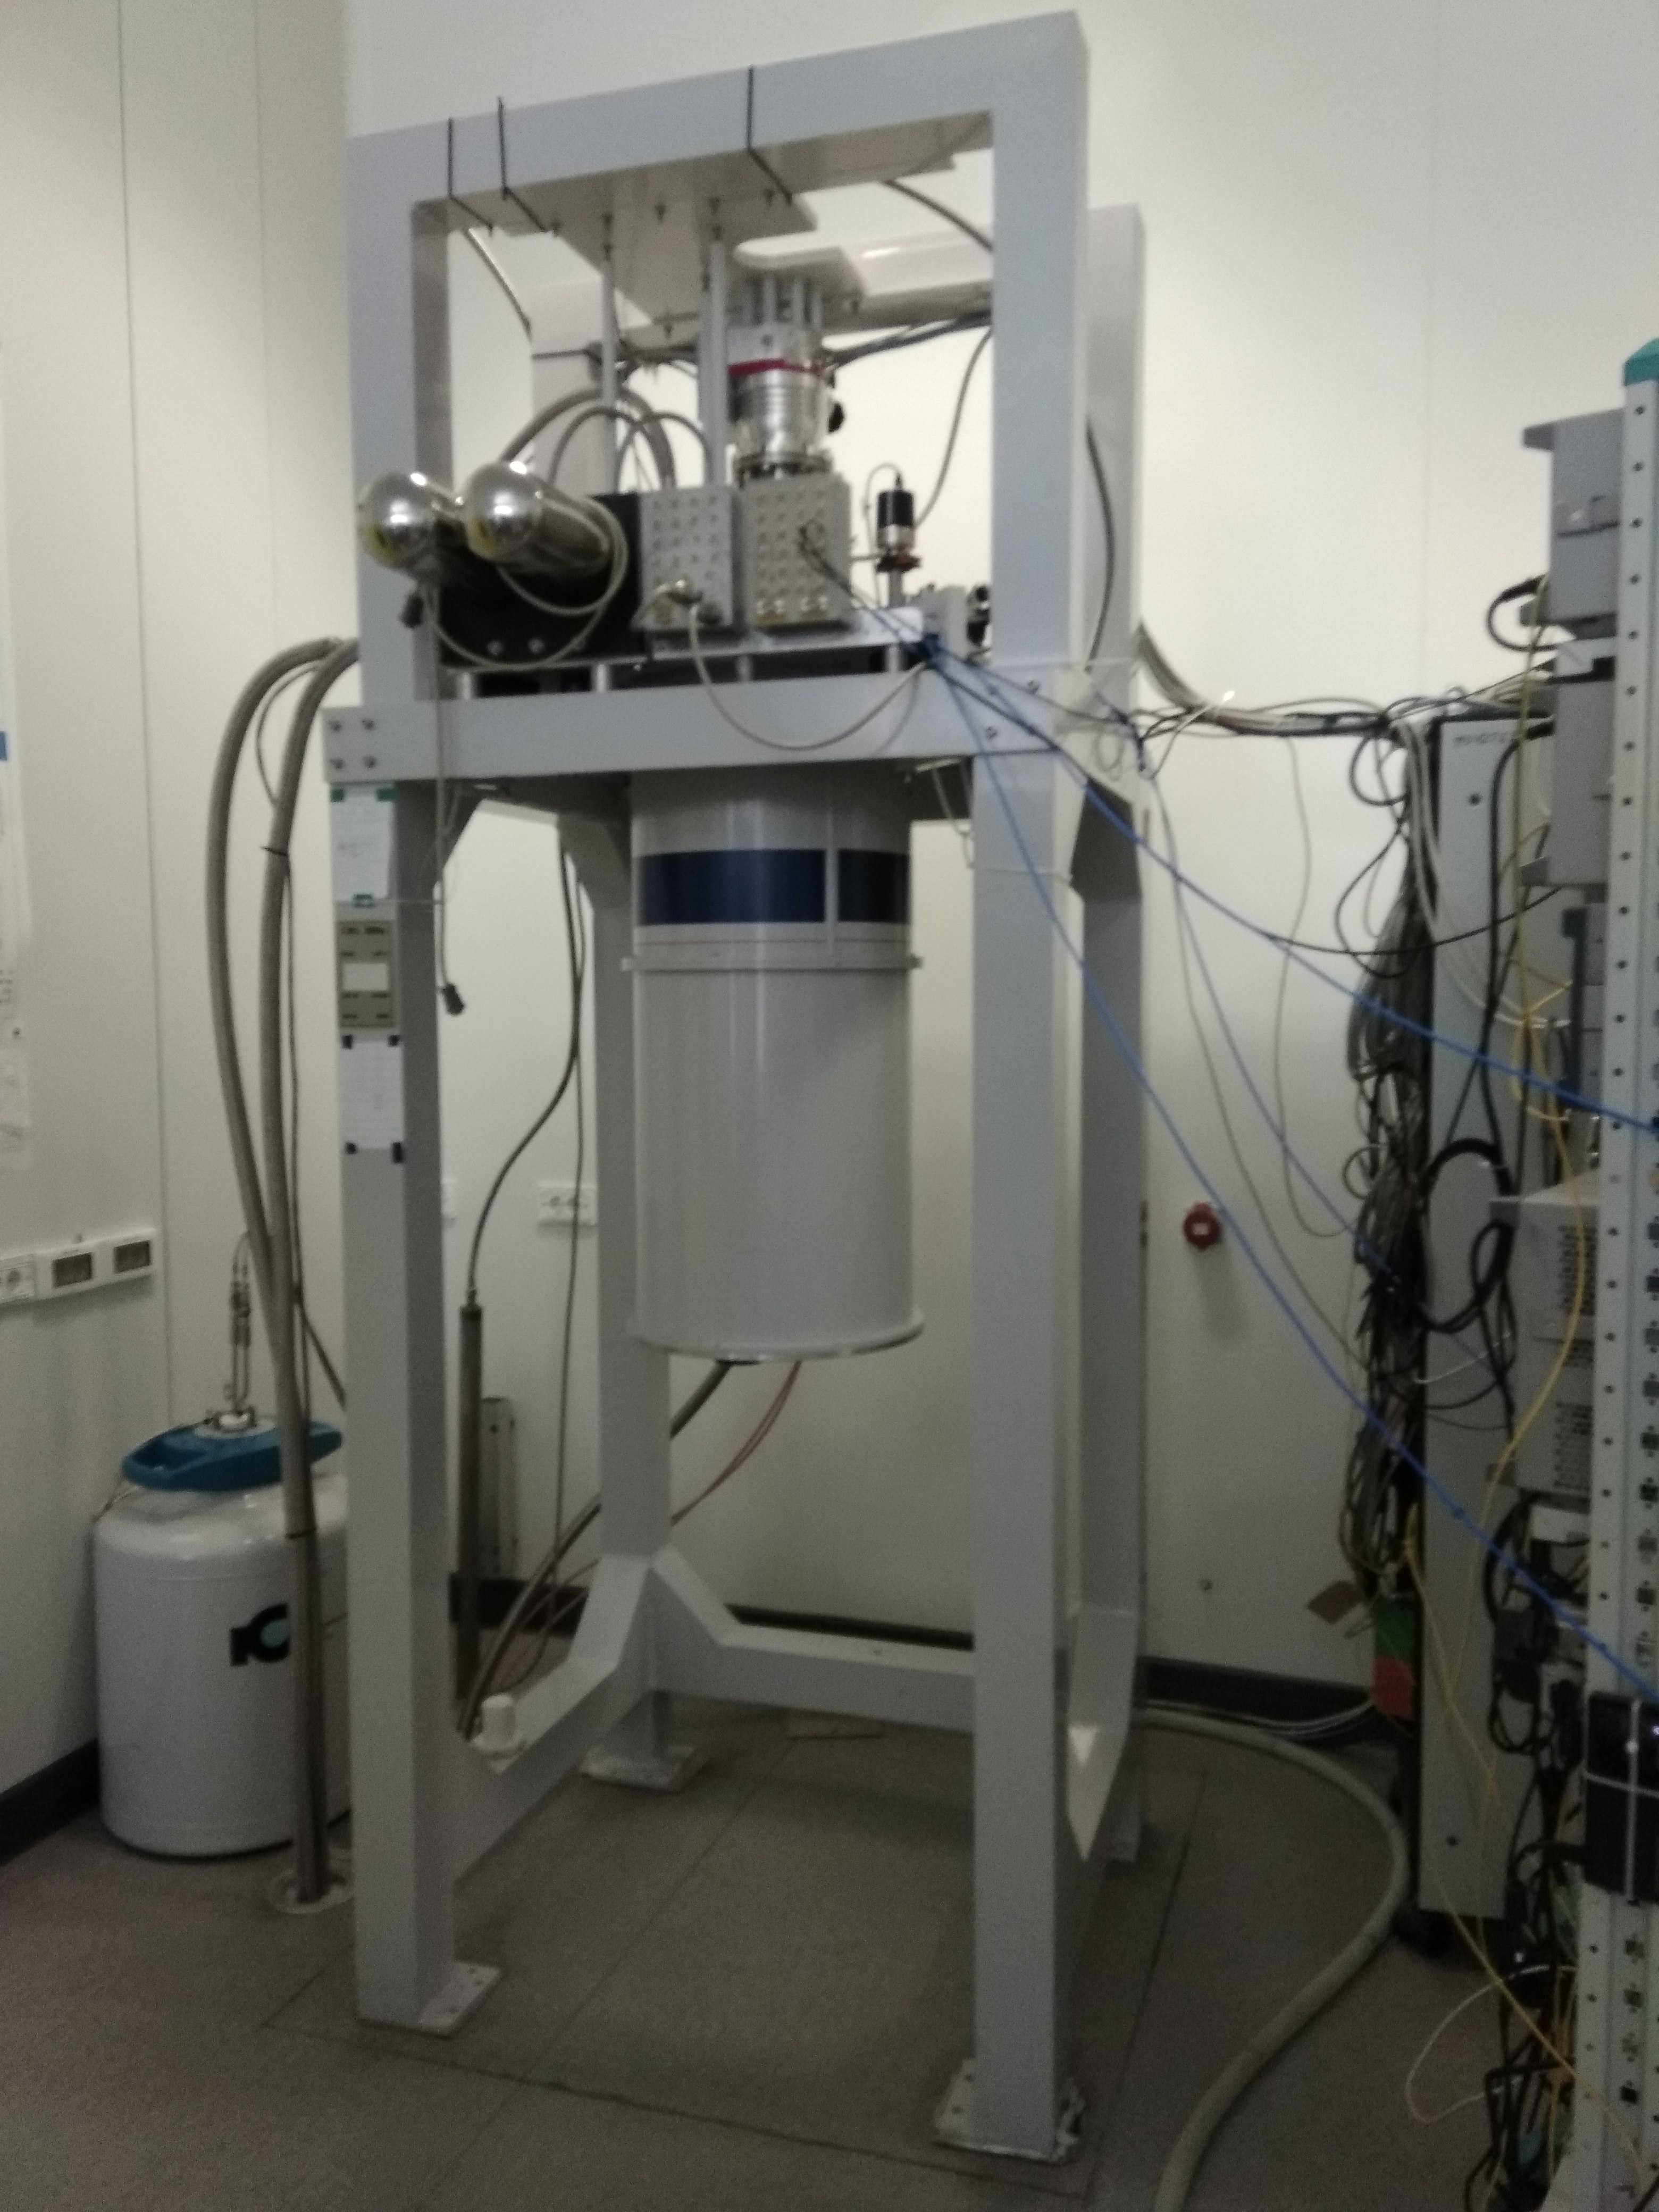
\includegraphics[width=0.9\linewidth]{pictures/IMG_20180614_120849} \\ а)}
	\end{minipage}
	\hfill
	\begin{minipage}[h]{0.49\linewidth}
		\center{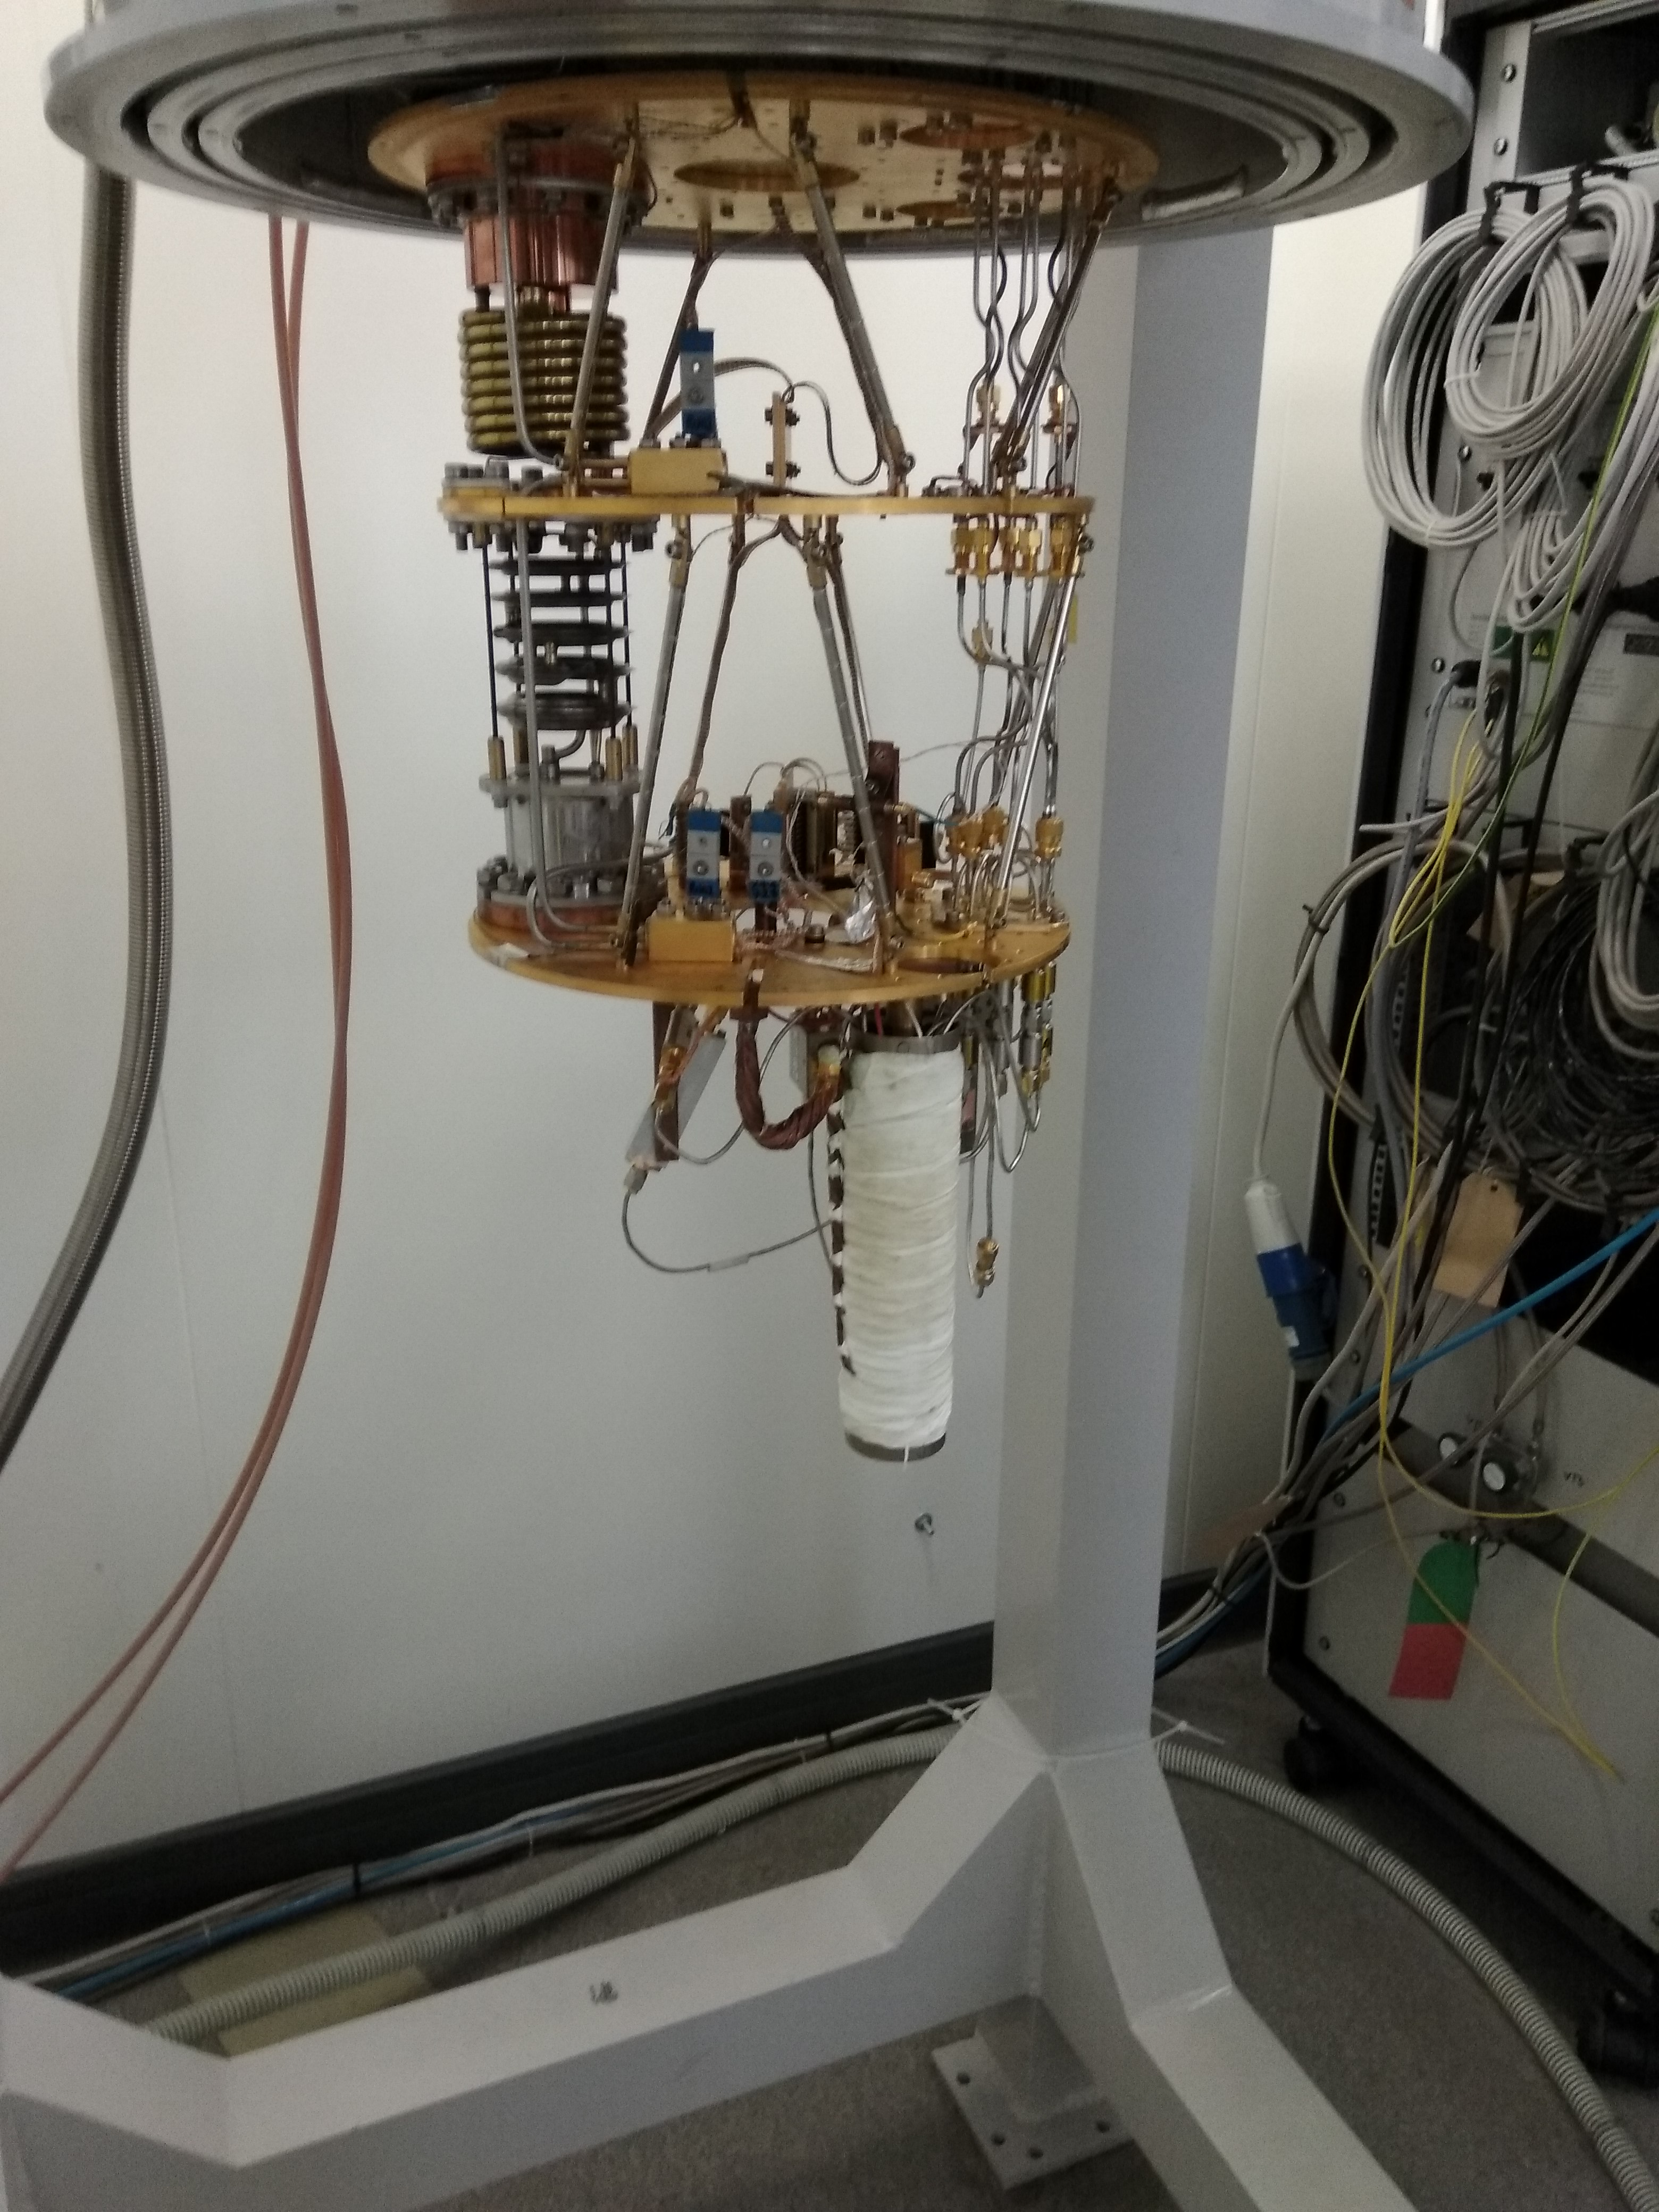
\includegraphics[width=0.9\linewidth]{pictures/IMG_20180614_123849} \\ б)}
	\end{minipage}
	\caption{Криостат растворения в закрытом (а) и открытом (б) видах}
	\label{ris:image1}
\end{figure}

Устройство состоит из турбомолекулярного насоса, для откачки паров ${^{3}He}$, компрессора для контроля криогенной системы, а так же вакуумной камеры, в которую и помещаются образцы. Вакуумная камера содержит несколько ступеней с последовательно усиливаемым охлаждением. Для минимизации теплообмена с окружающей система окружена экранами в виде концентрических цилиндров. Перед охлаждением систему откачивают до давления порядка $10^{-6}$ мбар. 

Т.к. воздействие на образец происходит посредством микроволновых сигналов, в криостат проведено 8 коаксиальных линий,а  так же медные провода для подачи постоянного тока.

В основе принципа работы лежит поглащение тепла при переходе фазы $^{3}He$ в $^{4}He$. На первом этапе происходит термо-акустическое охлаждение смеси  $^{3}He$ - $^{4}He$ до температуры порядка 700 мК. В силу того, что  $^{3}He$ легче, чем $^{4}He$ в результате этого процесса он оказывается сверху. Затем $^{3}He$ начинают откачивать, для того чтобы компенсировать потерю $^{3}He$ атомы вынуждены перемещаться в новые равновесные положения растворяясь при этом в смеси $^{3}He$ - $^{4}He$. Для того чтобы этот процесс происходил непрерывно в схему добавляется дополнительный импеданс для протекания процесса Джоуля - Томпсона для циркуляции смеси. Схема контура охлаждения представлена на Рисунке 17. 
\begin{figure}[h]
	\centering
	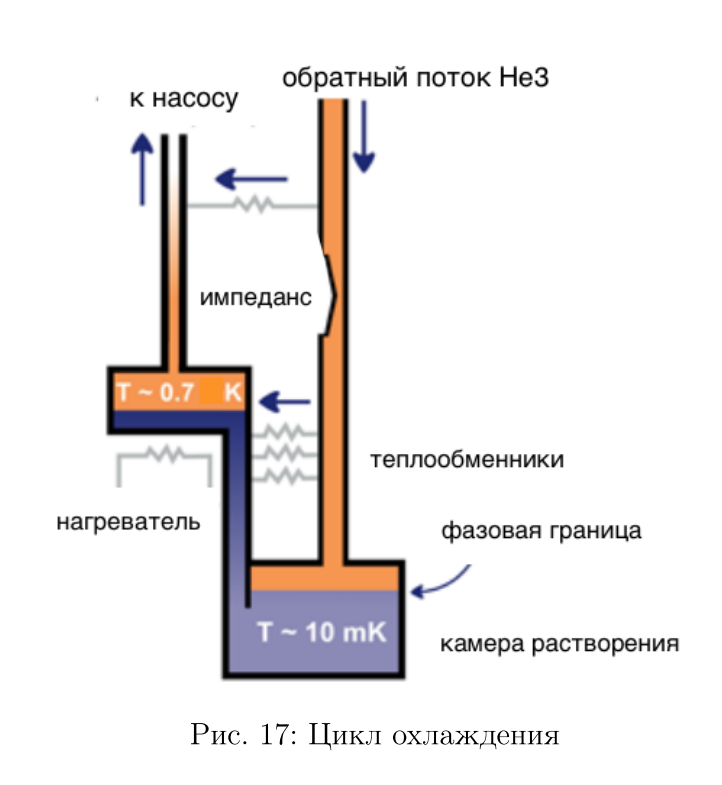
\includegraphics[width=0.5\linewidth]{pictures/fridgesheme}
	\caption{Схема контура охлаждения}
	\label{fig:fridgesheme}
\end{figure}
 
 \subsubsection {Аналого-цифровой преобразователь и ПЛИС}\label{adsfpga}
 Центральной частью данной работы было создание программного контроля для системы АЦП+ ПЛИС. АЦП (аналого-цифровой преобразователь) - устройство, преобразующее непрерывный аналоговый сигнал на входных каналах в дискретный цифровой. Для проведения экспериментов использовался 14-битный АЦП модели ADS54j40EVM компании Texas Instruments, частота дискретизации которого составляет 1000 сэмплов/сек. Модель представлена на Рисунке 18.
 
 \begin{figure}[!h]
 	\centering
 	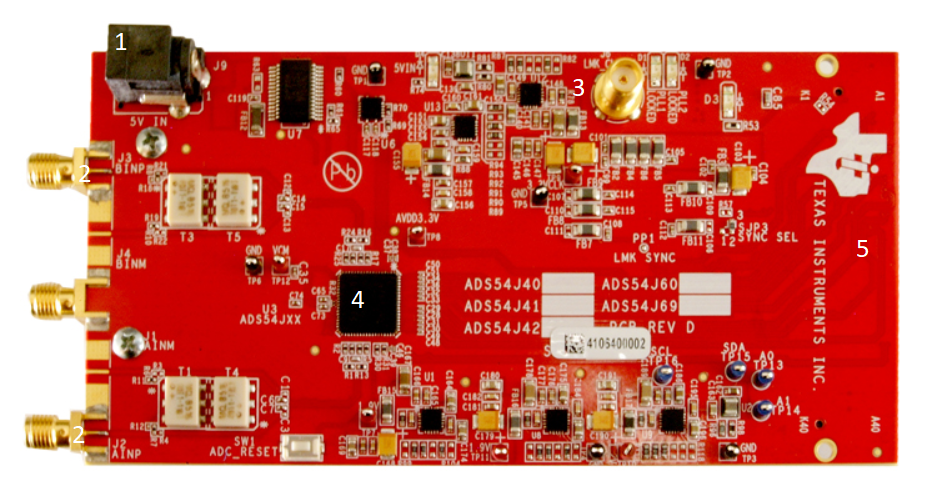
\includegraphics[width=0.7\linewidth]{pictures/ads}
 	\caption{ADS54j40EVM. Здесь 1 - канал питания, 2 - аналоговые входы, 3 - sma-разъём для синхронизирующего сигнала, 4 - чип с АЦП, 5 - разъём для связи с ПЛИС. Дополнительно на обратной стороны платы расположен тактовый генератор  }
 	\label{fig:ads}
 \end{figure}

ПЛИС (программируемая логическая интегральная схема) - полупроводниковое устройство, функционал которого генерируется пользователем уже после получения прибора. Программирование происходит путём изменения логики функционирования принципиальной схемы с помощью программирования на языке Verilog  и программного обеспечения Quartus Prime Software. Использование ПЛИС обусловлено значительно больше скоростью её работы по сравнению с обычными процессорами персональных компьютеров. Высокая скорость достигается в основном за счёт отсутствия ненужных в данной ситуации, интерфейсов, применяемых для общения с пользователем. Плата с ПЛИС TSW14J56EVM, использованной в работе, изображена на Рисунке 19.
\begin{figure}[h]
	\centering
	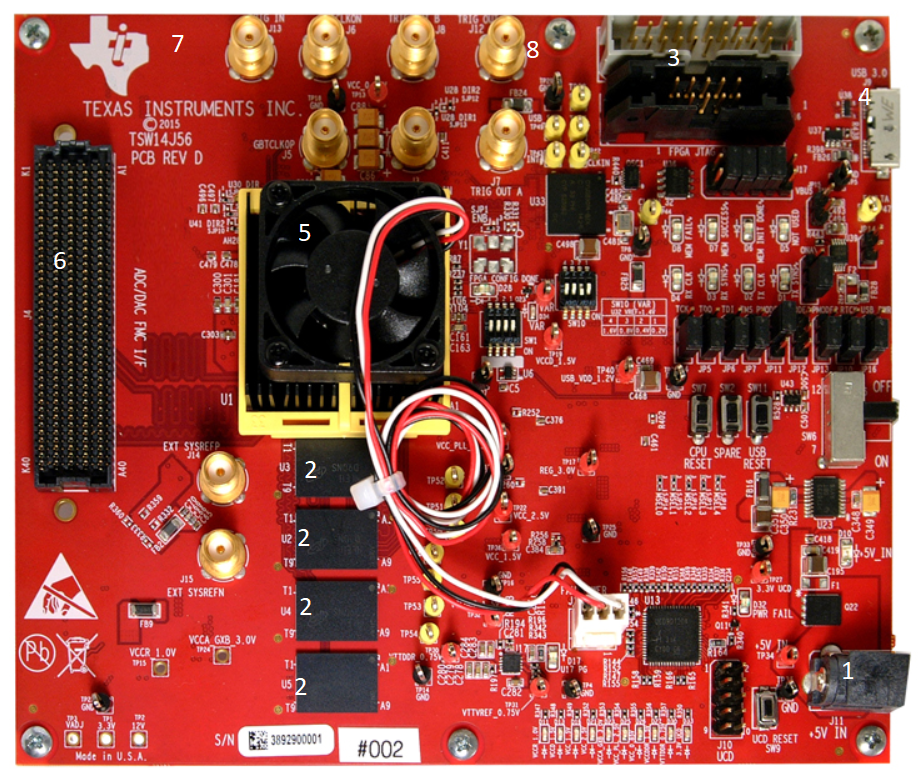
\includegraphics[width=0.5\linewidth]{pictures/fpga}
	\caption{ПЛИС TSW14J56EVM. Здесь 1 - канал питания, 2 - чипы с внешней памятью DDR, 3 - разъём JTAG для программирования ПЛИС, 4 - разъём USB для передачи данных с и на компьютер, 5 - чип с ПЛИС, 6 разъём для связи с АЦП, 7-8 каналы для получения и отправки триггеров во внешние устройства }
	\label{fig:fpga}
\end{figure}

Система ПЛИС+АЦП взаимодействует через JESD204b. Это интерфейс синхронной последовательной передачи больших объёмов данных. Суть его сводится к конвертации оцифрованного сигнала, представляющего собой значения на каждом из 14 бит каждого из двух каналов  АЦП в форму удобную для последующей обработке на ПЛИС а так же непосредственной передаче в виде последовательности 256-битных сегментов. 

На выходе JESD204b соединён со следующим виртуальным модулем, суть которого сводится к синхронному захвату данных из JESD, конвертации их в 256 бит в 512 и записи 512-битных сегментов в во внешнюю память. Следующая ступень, считывание из памяти и отправка данных по USB на ПК через интерфейс GPIF II. Синхронизация ПЛИС и АЦП обеспечивается интерфейсом JESD204b, а синхронизация АЦП и ПЛИС с внешними генераторами сигналов производится с помощью триггеров приходящих на аналоговые sma-разъёмы устройств.

\subsubsection{Схема экспериментальной установки}  
Помимо оцифровки сигнала и поддержания низких температур перед экспериментатором ставится ещё целый ряд задач, связанных в основном с генерированием сигналов правильной формы для считывания и контроля состояний кубитов. Для этих целей используются приборы, изображённый на Рисунке 20:

\begin{figure}[h]
	\centering
	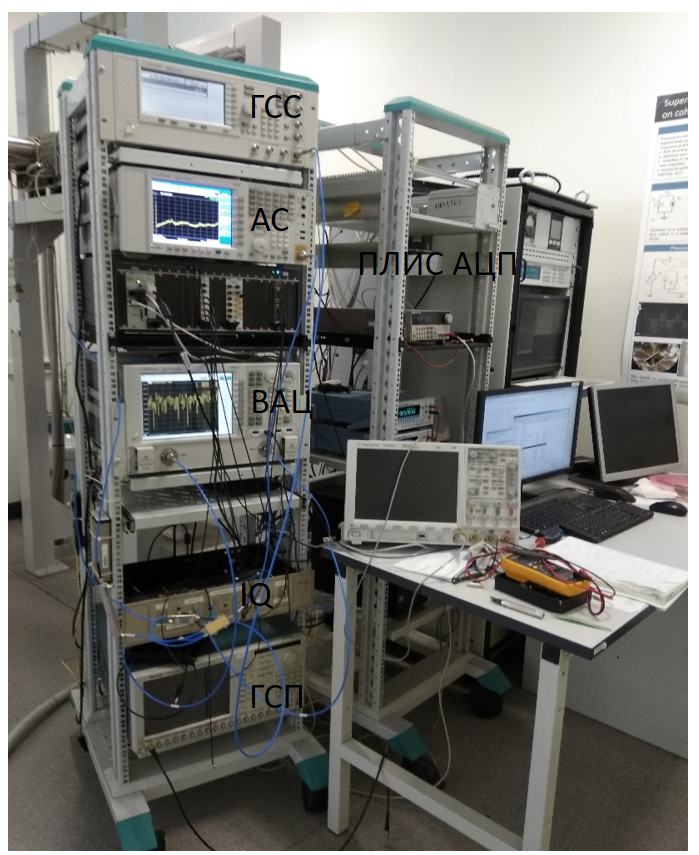
\includegraphics[width=0.6\linewidth]{pictures/shema1}
	\caption{Микроволновое оборудование}
	\label{fig:shema1}
\end{figure}


Всё это оборудование соединяется в специальную схему, дающую возможность генерировать как импульсный сигнал, для контроля и считывания состояний, так и непрерывный для проведения спектроскопии образцов. Здесь есть генератор высокочастотного синусоидального сигнала, анализатор спектров, векторный анализатор цепей, квадратурные смесители, генератор сигналов произвольной формы, осциллограф и АЦП+ПЛИС система. Всё это соединено по схеме, представленной на Рисунке 21. 

\begin{figure}[t!]
	\centering
	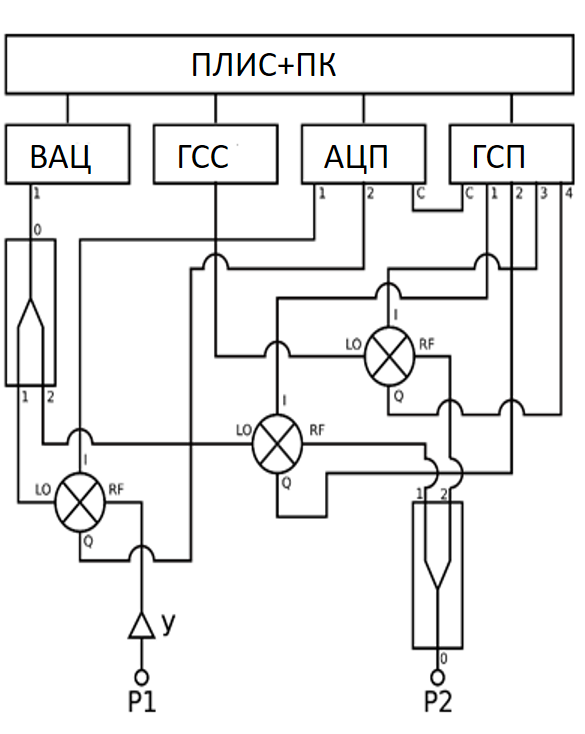
\includegraphics[width=0.5\linewidth]{pictures/shema}
	\caption{Схема соединения экспериментального оборудования}
	\label{fig:shema}
\end{figure}

\subsection{Спектроскопия образцов}
\subsubsection{Однотоновая спектроскопия}\label{sigletone}
Очевидно, что для манипуляции и считывания кубитных состояний нужно знать, на какой частоте подавать сигналы. Поэтому любые измерения начинаются с поиска спектров резонатора и кубитов. Как было сказано в (\ref{transmon}) используя СКВИД можно перестраивать частоту перехода кубита в зависимости от внешнего магнитного потока. Частота резонатора при этом не меняется. Для проведения однотоновой спектроскопии  последовательно подаётся сигнал на разных частотах и меняется внешний магнитный поток с использованием постоянного тока. В результате получается зависимость коэффициента прохождения на ВАЦ от внешнего потока и частоты сигнала, как изображено на Рисунке 22. 

Частота кубита косинусоидально зависит от внешнего потока, поэтому на Рисунке 22 видно пересечение прямой линии, отвечающей резонатору с косинусоидальной, отвечающей кубиту. В точках пересечения наблюдается вырождение состояний отвечающих нахождению фотона в кубите и в резонаторе. 

\begin{figure}[t]
	\centering
	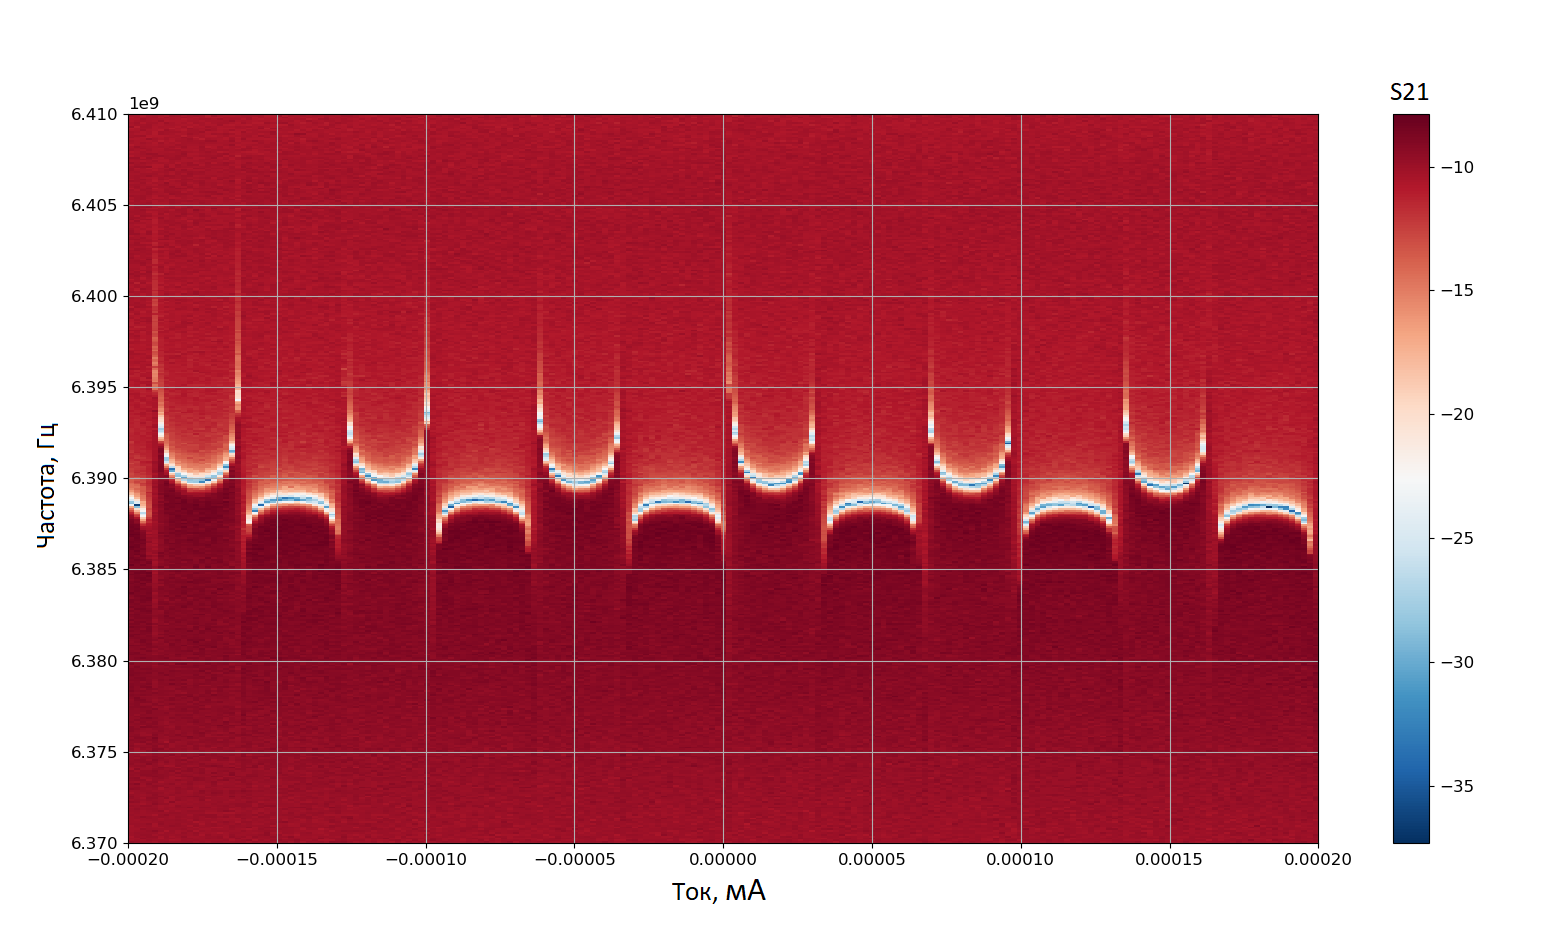
\includegraphics[width=0.9\linewidth]{pictures/anticross_6_39}
	\caption{Однотоновая спектроскопия}
	\label{fig:anticross639}
\end{figure}

Точки вырождения на однотоновом спектре обычно называют антикроссингами или квазипересечениями. Они дают информацию о том, при каком токе стоит искать минимум и максимум частоты кубита. Стоит заметить, что все воздействия на перестраиваемые кубиты происходят или в максимуме или в минимуме частоты, потому что там кубит менее восприимчив к потоковым шумам. 

\subsubsection{Двухтоновая спектроскопия}
Определившись со значениями частоты резонатора и тока для максимальных и минимальных частот кубита, можно переходить к двухтоновой спектроскопии. Результат измерения представлен на Рисунке 22: 
\begin{figure}[!h]
	\centering
	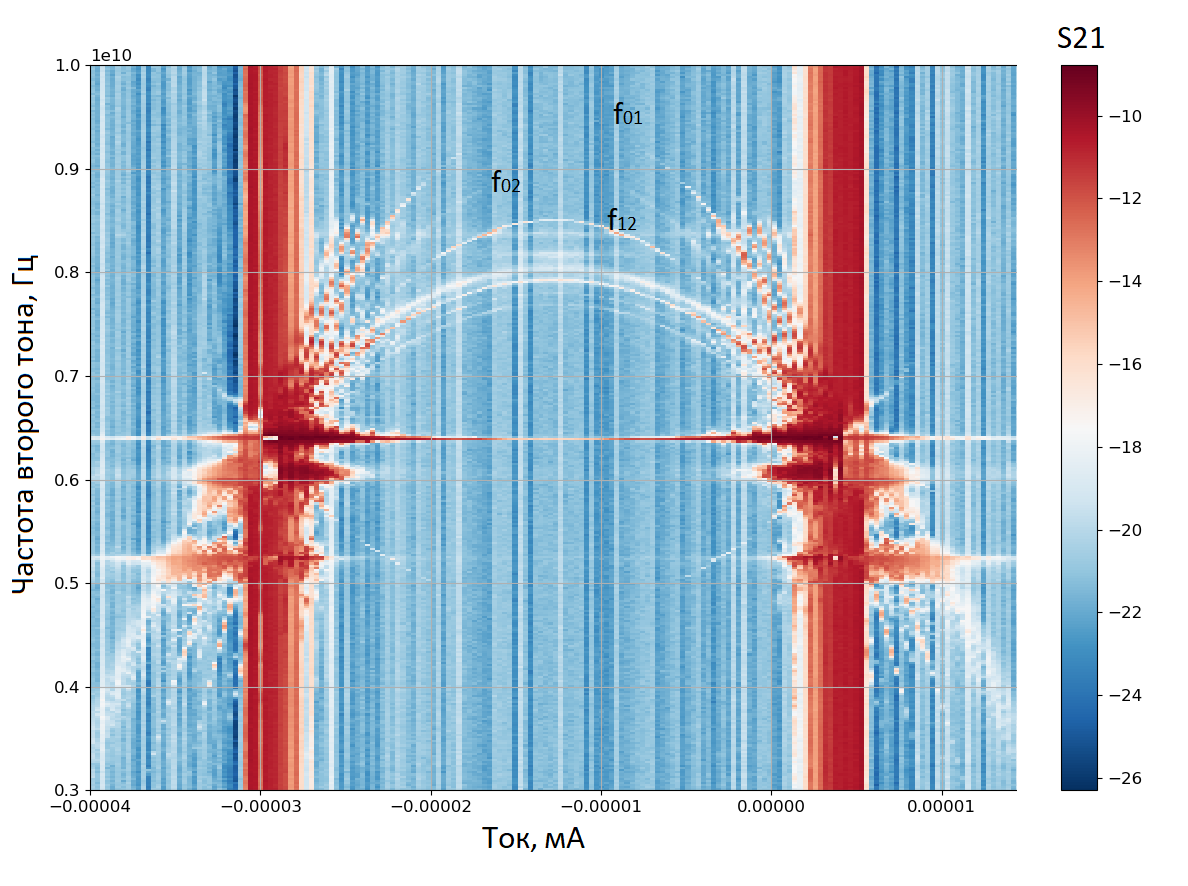
\includegraphics[width=0.8\linewidth]{pictures/2tone6_39}
	\caption{Двухтоновый спектр}
	\label{fig:2tone639}
\end{figure}

Принцип её работы основан на эффекте описанном в (\ref{transres}), В отличие от однотоновой спектроскопии здесь присутствует два сигнала. Один генерируется на частоте, равной частоте резонатора, найденной в (\ref{sigletone}), второй в некотором диапазоне частот, в которую, предположительно входит максимальная частота кубита. Перестраивая частоту кубита постоянным, можно наблюдать косинусоидальную линию, соответствующую кубиту, и прямую линию соотвествующую резонатору. Стоит заметить, что спектроскопия проводилась при большой мощности кубитного тона и потому на спектре видно сразу несколько переходов в трансмоне. 

\subsection{Импульсные измерения}
\subsubsection{Осцилляции Раби}

Импульсные измерения кубитов начинаются с наблюдений осцилляций Раби, подобно тому, как это было описано в (\ref{cohdin}). Для этого с помощью квадратурных смесителей и генератора сигналов произвольной формы из непрерывного синусоидального сигнала вырезаются прямоугольные импульсы и отправляются на образец. Затем посылается считывающий сигнал. Последовательность импульсов изображена на Рисунке 23.
\begin{figure}[h]
	\centering
	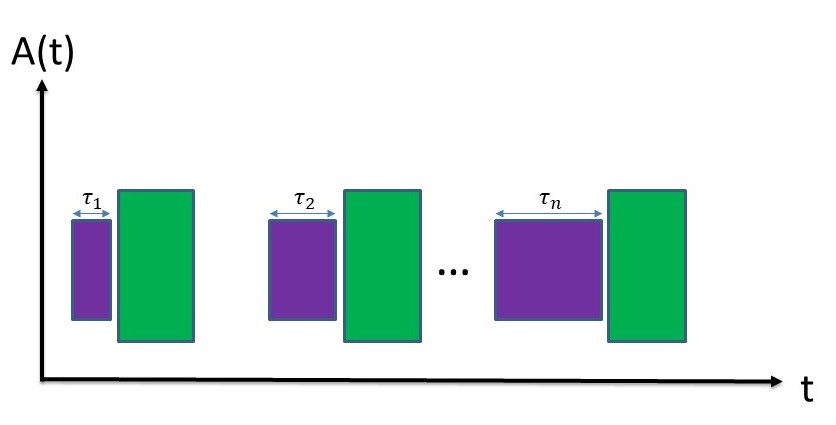
\includegraphics[width=0.6\linewidth]{pictures/Rabipulseseq}
	\caption{Последовательность импульсов для наблюдения осцилляций Раби. Зелёным цветом изображён импульс на частоте резонатора, а фиолетовым на частоте кубита}
	\label{fig:rabipulseseq}
\end{figure}

Как видно из Рисунка 23,  длительность возбуждающего кубит импульса $\tau_i$ меняется в некотором диапазоне значений. В результате такой последовательности наблюдается картина изображённая на Рисунке 24. Данные аппроксимируются функцией вида $e^{-\frac{t}{t}} \sin{\omega_r t}$, где $\omega_r$ это частота Раби-осцилляций. Знание Раби-частоты даёт информацию о длительности сигнала, необходимого для перевода кубита из одного состояния в другое. 

Так например время $\pi$- импульса, т.е. импульса под действием которого квантовое состояние совершает поворот на $180^{\circ}$, составляет половину Раби-периода.
\clearpage

\begin{figure}[h]
	\centering
	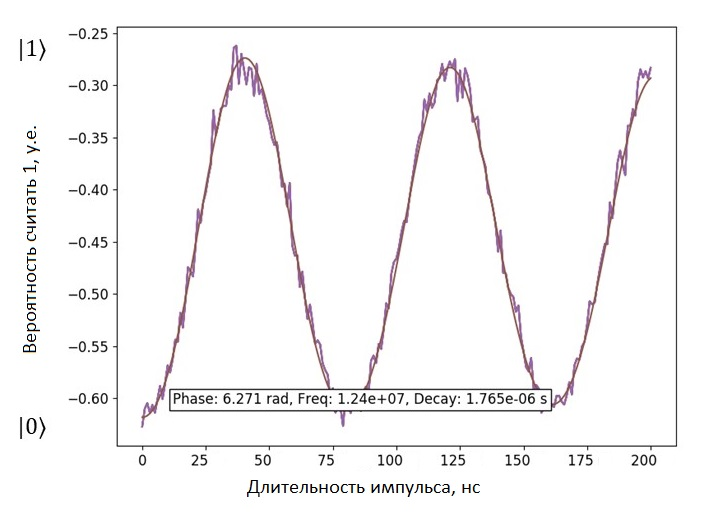
\includegraphics[width=0.7\linewidth]{pictures/rabires.png}
	\caption{Раби осцилляции. Фиолетовым цветом - экспериментальные данные, коричневым - подгоночная кривая}
	\label{fig:rabires}
\end{figure}


\subsubsection{Время когерентности и релаксации}
Как было показано в  (\ref{neun}) взаимодействие с окружением разрушает чистое квантовое состояние, переводя его в смешанное. Для того чтобы обладать информацией о длительности того промежутка времени, в течение которого кубит пригоден для проведения квантовых алгоритмов измеряются два характерных параметра.

Первый параметр - время когерентности, т.е. время, за которое квантовое состояние становится из максимально чистого максимально смешанным под действием дефазировки. Эксперимент по измерению этого времени называется наблюдением осцилляций Рамзи. Импульсная последовательность для этого случая изображена на Рисунке 26:

\begin{figure}[h]
	\centering
	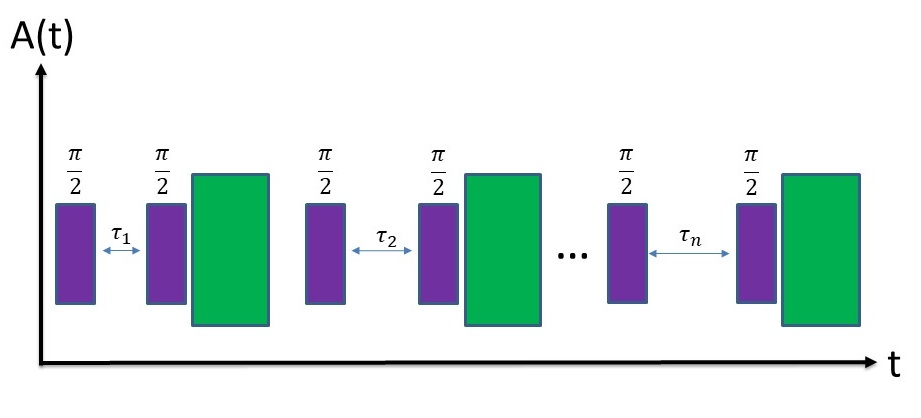
\includegraphics[width=0.6\linewidth]{pictures/Ramseypulseseq}
	\caption{Последовательность импульсов при наблюдении осцилляций Рамзи}
	\label{fig:ramseypulseseq}
\end{figure}

 Суть её заключается в следующем. На кубит подётся $\frac{\pi}{2}$ - импульс, который переводит квантовое состояние на экватор сферы Блоха. Там, как было показано в (\ref{neun}) ввиду наличия дефазировки состояние начинает свободную прецессию вдоль экватора. После задержки $\tau$, величина которой варьируется от нуля до некоторого параметра, подаётся второй $\frac{\pi}{2}$. Естественно, если задержки между импульсами не было, то два $\frac{\pi}{2}$ импульса эквивалентны одному $\pi$, в таком случае кубит окажется в состоянии $|1\rangle$. Но если вектор состояния прошёл половину экватора сферы Блоха, переместившись, к примеру, из состояния $|+\rangle$ в состояние $|-\rangle$, второй $\frac{\pi}{2}$-импульс переведёт его обратно в состояние $|0\rangle$. Итоговый график изображён на Рисунке 27:
 
 \begin{figure}[h]
 	\centering
 	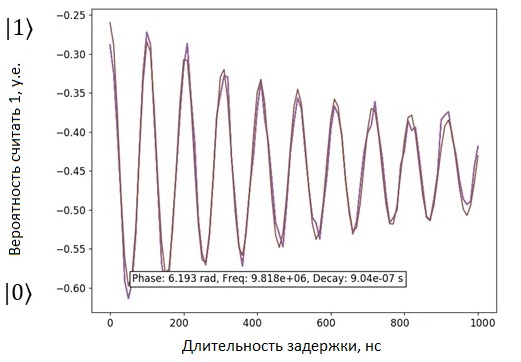
\includegraphics[width=0.7\linewidth]{pictures/ramseyres.png}
 	\caption{Осцилляции Рамзи. Фиолетовый цвет - экспериментальные данные, коричневый - подгоночная кривая}
 	\label{fig:ramseyres}
 \end{figure}

Результат аппроксимируется функцией вида $e^{-\frac{t}{T_2}}\sin{\omega t}$, здесь $T_2$ - время когерентности кубита,т.е. время, за которое вероятность считать $|1\rangle$ после второго $\frac{\pi}{2}$-импульса уменьшилась в e раз, а частота этих осцилляций равна отстройке частоты сигнала от частоты кубита. Используя этот параметр, можно точнее подбирать частоту сигнала для контроля квантового состояния. 

Второй параметр - время релаксации $T_1$. Физическая величина, отражающая скорость распада перехода кубита из чистого состояния $|1\rangle$ в смешанное состояние равновесия. Импульсная последовательность представлена на Рисунке 28.

\begin{figure}[h]
	\centering
	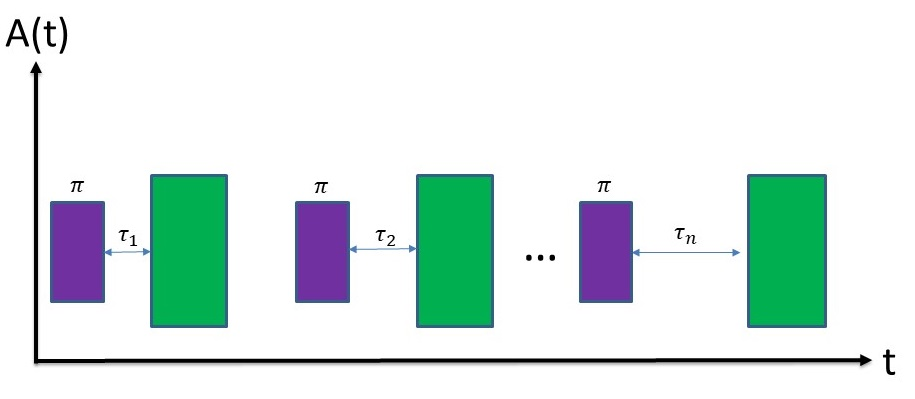
\includegraphics[width=0.6\linewidth]{pictures/todinpulseseq}
	\caption{Последовательность импульсов для определения времени релаксации}
	\label{fig:todinpulseseq}
\end{figure}

В этом эксперименте необходимо перевести кубит в состояние $|1\rangle$ и через некоторый промежуток времени послать считывающий импульс. Производится скан по величине промежутка. Результат представлен на Рисунке 29.

\begin{figure}[h]
	\centering
	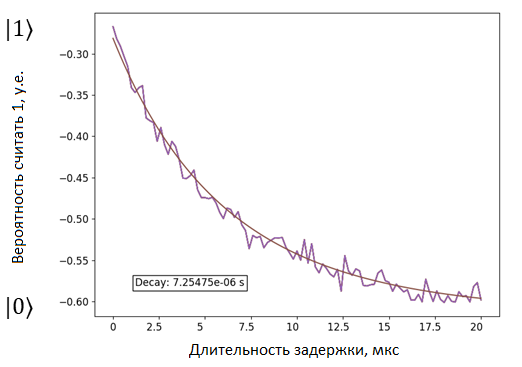
\includegraphics[width=0.7\linewidth]{pictures/t1res.png}
	\caption{Релаксация квантового состояния.Фиолетовым цветом - экспериментальные точки, коричневым подгоночная кривая}
	\label{fig:t1res}
\end{figure}

В этот раз данные фитуются затухающей экспонентой, а время релаксации - величина обратная декременту затухания. 

\subsection {Дискриминация квантовых состояний}\label{discr}
Одной из задач машинного обучения является так называемая задача статистической классификации. Она состоит в присваивании произвольной выборке значений определённого класса в зависимости от статистических характеристик данной выборки. Компьютерные алгоритмы решения такого рода задач широко используются в медицине, геолого-разведочных операция и целом ряде других задач. Не является исключением и экспериментальная квантовая информатика, в которой задача классификации используется при считывании.

После определения частот и длительностей возбуждающих и считывающих сигналов, а так же характерных времён, в течение которых возможно оперирование квантовой системой можно приступить к ряду новых задач. Одной из таких задач является единовременное считывание квантового состояния (Single shot readout).  

Концепция такого считывания состоит в следующем. На кубит посылается считывающий импульс. Как всегда по кабелям он доходит до чипа, проходит по передающей линии или уходит в резонатор в зависимости от состояния кубита. Так или иначе, на выходе из криостат результат приходит на АЦП. Как было указано ранее (\ref{adsfpga}) такой результат представляет собой развёртку значений напряжений во времени. И внешний вид напряжения, как функции времени напрямую зависит от состояния кубита. Пример такой зависимости представлен на Рисунке 30.


\begin{figure}[h]
	\centering
	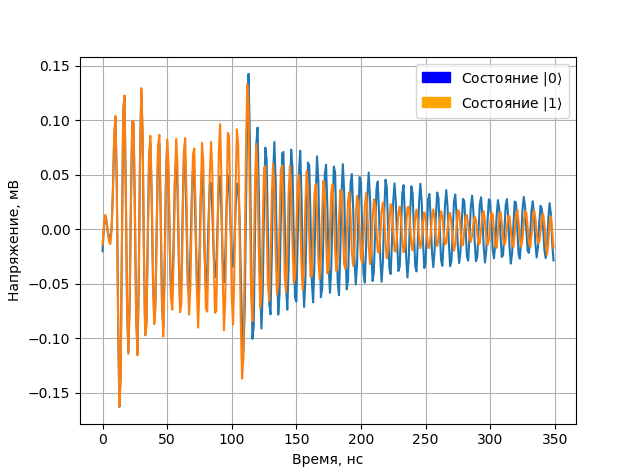
\includegraphics[width=0.7\linewidth]{pictures/Etalones}
	\caption{Вид считывающих импульсов соответствующих разным квантовым состояниям}
	\label{fig:etalones}
\end{figure}

С точки зрения задачи классификации каждый такой считывающий импульс представляет собой некоторую статистическую выборку. И каждому из них необходимо присвоить класс, (в данном случае класс $|0\rangle$ и $|1\rangle$) и, следовательно считать состояние. 

В работе использовалось два классификатора. Первым из них был линейный дискриминатор (LDA). Процесс обучения состоял из ряда этапов. С заранее известным состоянием производится 50000 повторений записи значений напряжения для каждого из классов. Далее случайные $70 \%$ от общего числа записей отделяются. Для них считается среднее напряжение как функция времени:

\begin{equation}
\tag{41}
\mu(t) = \frac{1}{n}\sum_{n=1}^{35000} V_n(t)
\\
\end{equation}

На этом процесс обучения линейного дискриминатора заканчивается и начинается процесс тестирования. Для каждой из оставшихся выборок считается разность коэффициентов ковариации с $\mu_0(t)$ и $\mu_1(t)$.

\begin{equation}
\tag{42}
K_n = \langle V_n\rangle\langle\mu_0(t)\rangle - \langle V_n\rangle\langle\mu_1(t)\rangle
\\
\end{equation}

При этом если величина $K_n$ положительна, состояние классифицируется, как $|0\rangle$, а если отрицательна - как $|1\rangle$. 

Вторым классификатором был квадратичный (QDA). В этом случае на тренировочной выборке помимо среднего значения считается так же ковариационная матрица:
\begin{equation}
\tag{43}
\Sigma_{ij} = cov(X_i,X_j)
\end{equation}

Здесь $X_i$- вектор размерности выборки. Т.е. по существу, это матрица, которая показывает, величину дисперсии определения значения в каждой точке по времени.

В случае QDA формула классификации имеет вид:
\begin{equation}
\tag{45}
Q_n = -\frac{1}{2}V^T(\Sigma_0^{-1}- \Sigma_1^{-1})V+ V^T(\Sigma_0^{-1}\mu_0- \Sigma_1^{-1}\mu_1)
\end{equation}
А величина порога, которая для LDA являлась нулём, считается из соотношения:
\begin{equation}
\tag{46}
Q_{tresh}= \frac{1}{2}(\mu_0^T\Sigma_0^{-1}\mu_0 - \mu_1^T\Sigma_1^{-1}\mu_1)+\frac{1}{2}\log{\frac{|\Sigma_0|}{|\Sigma_1|}}
\end{equation}
Здесь $|\Sigma_i|$ - определители матриц. 

Соотвественно, если величина $Q_n$ больше, чем $Q_{tresh}$, то состояние классифицируется как $|0\rangle$, в противном случае как $|1\rangle$.Критерием считывания в простейшем случае является величина фиделити, определяемая из формулы:
\begin{equation}
\tag{47}
F = 1 -\frac{N_{FP}+N_{FN}}{2},
\end{equation}
\noindent где $N_{FP}$ и $N_{FN}$ число неправильно определённых состояний $|0\rangle$  и $|1\rangle$ соотвественно. Фиделити линейного дискриминатора оказалось 75 \%, а фиделити QDA о 83 \%.

Результирующая гистограмма представлена на Рисунке 31:

\begin{figure}[h]
	\centering
	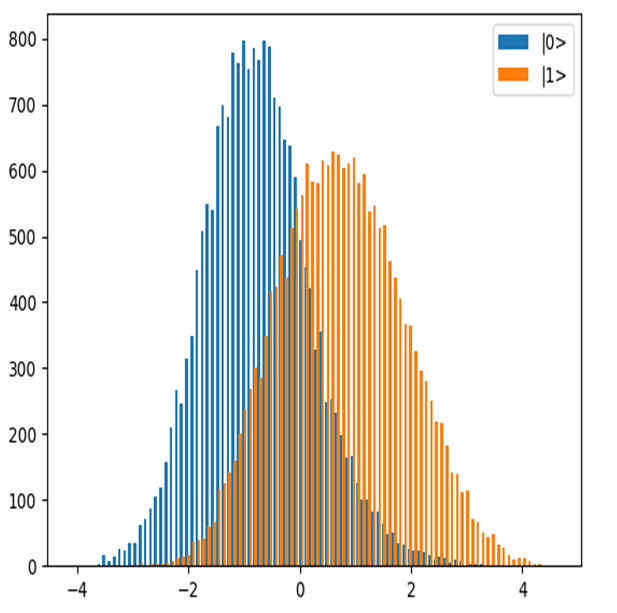
\includegraphics[width=0.5\linewidth]{pictures/resulthist}
	\caption{Гистограмма квантовых состояний $|0\rangle$ и $|1\rangle$}
	\label{fig:resulthist}
\end{figure}
\clearpage
\subsection{Двойное считывание}\label{doubleread}
С точки зрения считывания остался ещё один вопрос, на который пока не было дано ответа. В случае ошибки дискриминации, как понять, развалилось ли состояние до считывания или произошла ошибка классификации из-за наложившихся на сигнал шумов. Ответ на этот вопрос поможет найти двойное считывание.

Схема его состоит в следующем. На кубит в исходном состоянии $|0\rangle$ подаётся два считывающих импульса с варьируемой задержкой. Затем считается коэффициент их ковариации друг с другом, как функция задержки. Результат изображён на Рисунке 32:

\begin{figure}[h]
	\centering
	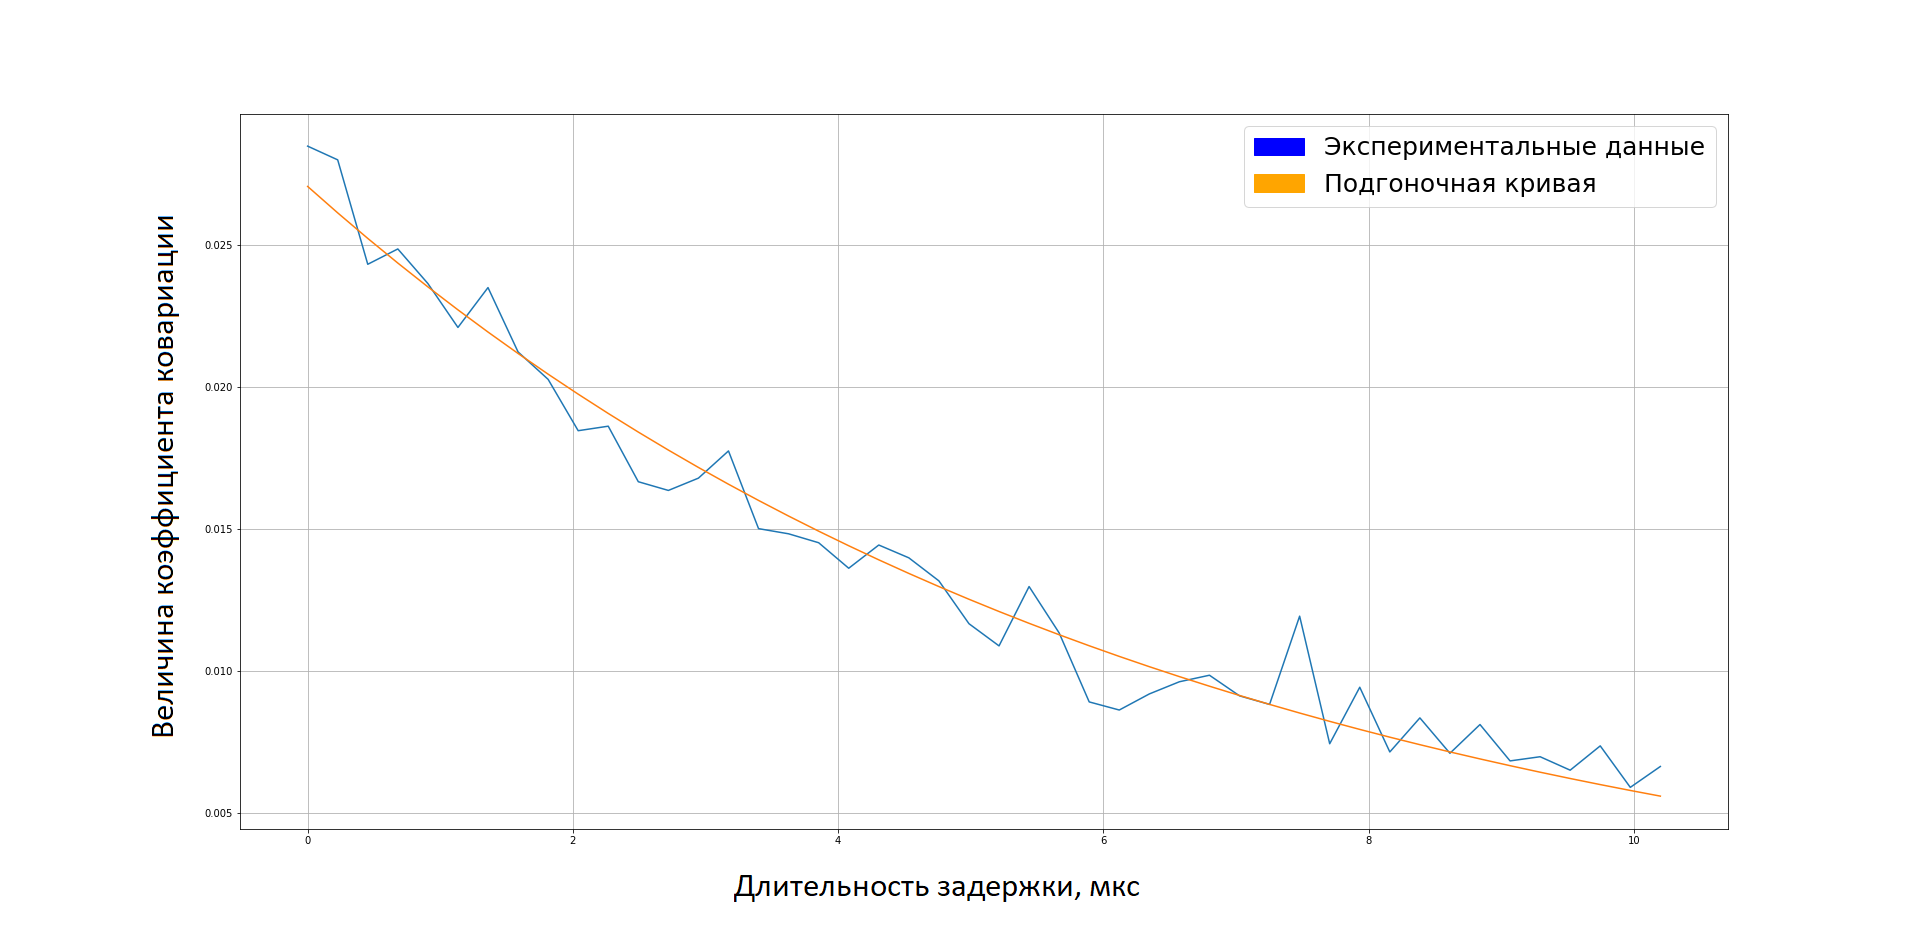
\includegraphics[width=0.8\linewidth]{pictures/result}
	\caption{Ковариация последовательных считывающих импульсов }
	\label{fig:result}
\end{figure}

Из этого графика можно получить три важных параметра, значение ковариации в первый момент времени, когда между импульсами не было задержки,декремент экспоненциального затухания и среднее значение состояния.

Далее составляется модель ошибок. Если считать, что существует только два типа ошибок – ошибка приготовления состояния (в дальнейшем $P_0$) и ошибка считывания ($P_r$). Первая ошибка – по причинам взаимодействия с тепловым окружением кубит изначально оказался в состоянии $|1\rangle$. Вторая ошибка – несмотря на то, что на самом деле кубит был в состоянии $|0\rangle$ в процессе обработки шумного сигнала он был классифицирован, как $|1\rangle$. В этом случае вероятности считать $|0\rangle$ и $|1\rangle$ в первом измерении вычисляются по формулам:
\begin{equation}
\tag{48}
\begin{split}
&P(Q_1 = 0)= 1- P_0 - P_r +P_0P_r\\
&P(Q_1 = 1)= P_0+P_r - P_0P_r
\end{split}
\end{equation}

Теперь надо подумать, что будет происходить с вероятностями двойного считывания. Во-первых, вероятность второй раз считать кубит в $|1\rangle$  если и первый раз он был в $|1\rangle$ должна в начальный момент времени быть равна 1-$P_r$ т.к. считать не единицу можно только  в случае ошибки считывания. А на больших временах, вероятность считать единицу складывается из вероятности ошибки считывания (из-за процессов некогерентной релаксации), ошибки приготовления (прошло какое-то время, в течение которого кубит находился в тепловом равновесии с окружением), за вычетом их произведения (так как, совершив обе ошибки,результат не изменится).

\begin{equation}
\tag{49}
\begin{split}
P(Q_2 = 1 | Q_1 = 1) &= e^{-\gamma t}(1-P_0 - P_r +P_0P_r-P_r)+ P_r +P_0-P_0P_r = \\
&e^{-\gamma t}(1-P_{relax}-P_r)+P_{relax},
\end{split}
\end{equation}
\noindent где $P_{relax} = P_r +P_0-P_0P_r$, а $\gamma$ коэффициент затухания ковариации последовательных считывающих импульсов.Соответственно, вероятность считать состояние $|0\rangle$ сразу после $|1\rangle$ выражается формулой:

\begin{equation}
\label{ubi}
\tag{50}
P(Q_2 = 0 | Q_1 = 1)= 1- e^{-\gamma t}(1-P_{relax}-P_r)+P_{relax}
\end{equation}

Чтобы найти вероятность состояния $|1\rangle$ при втором считывании, если результатом первого был $|0\rangle$ ,в  выражении (\ref{ubi}) $P_{relax}$ заменяется на $1-P_{relax}$:

\begin{equation}
\tag{51}
P(Q_2 = 1 | Q_1 = 0)= P_{relax} - e^{-\gamma t}(P_{relax}-P_r)+P_{relax}
\end{equation}

А для вероятности считать $|0\rangle$  второй раз,при первом исходе-$|0\rangle$:

\begin{equation}
\tag{51}
P(Q_2 = 0 | Q_1 = 0)= 1 - P_{relax} + e^{-\gamma t}(P_{relax}-P_r)
\end{equation}

 Для математического описания полученной экспериментальной зависимости и для извлечения из неё искомых вероятностей ошибок необходимо посчитать ковариацию этих двух считываний ($Q_1$  и $Q_2$ ):
 
 \begin{equation}
 \label{cov}
 \tag{52}
 Cov_{Q_1Q_2} = \langle Q_1 Q_2 \rangle - \langle Q_1\rangle\langle Q_2\rangle
 \end{equation}
 
Где $\langle Q_1 Q_2 \rangle = P_{relax}(e^{-\gamma t}(1-P_{relax}-P_r)+P_{relax})$ это среднее значение произведения результатов считываний, посчитанное, как произведение $P(Q_1 = 1) P(Q_2 = 1|Q_1 = 1)$. Значение $\langle Q_1 \rangle = P_{relax}$, а $\langle Q_2 \rangle$:
\begin{equation}
\tag{53}
\langle Q_2 \rangle = P(Q_1 = 1| Q_2 =1) + P(Q_1 = 1| Q_2 = 0)=
P_{relax}+P_re^{-\gamma t}-2P_{relax}P_re^{-\gamma t}
\end{equation}
Наконец, подстановка в (\ref{cov}) даёт следующий результат:
\begin{equation}
\tag{54}
Cov_{Q_1Q_2}= P_{relax}e^{-\gamma t}-P_{relax}^2e^{-\gamma t}+2P_rP_{relax}^2e^{-\gamma t}- 2P_re^{-\gamma t}
\end{equation}
Подстановка среднего значения дискриминатора и коэффициента ковариации в перый момент времени приводит к системе из двух уравнений из которых можно выразить искомые величины:
\begin{equation}
\tag{55}
\begin{split}
&P_r = \frac{Cov_0+P_{relax}^2-P_{relax}}{2P_{relax}^2-2}\\
&P_0 = \frac{P_{relax} - P_r}{1-P_r}
\end{split}
\end{equation}

В данной работе ошибка инициализации составила 20 \% , а ошибка считывания 8 \%.
\subsection{Обратная связь}
Результат вычислений, приведённых в главе (\ref{doubleread}) наводит на мысль о том, что раз ошибка инициализации большем ошибки считывания, то имеет смысл придумать способ корректировать начальное состояния. Задача однако усложняется тем, что необходимо провести единовременное считывание и корректирующее воздействие за времена много меньшие времён когерентности и релаксации, которые как было показано в составляют 0.9 и 7.1 мкс соответственно. Здесь и раскрывается весь потенциал системы ПЛИС+АЦП описанной в (\ref{adsfpga}). 

Схема эксперимента пл созданию так называемой обратной связи представлена на Рисунке 33:
\begin{figure}[h]
	\centering
	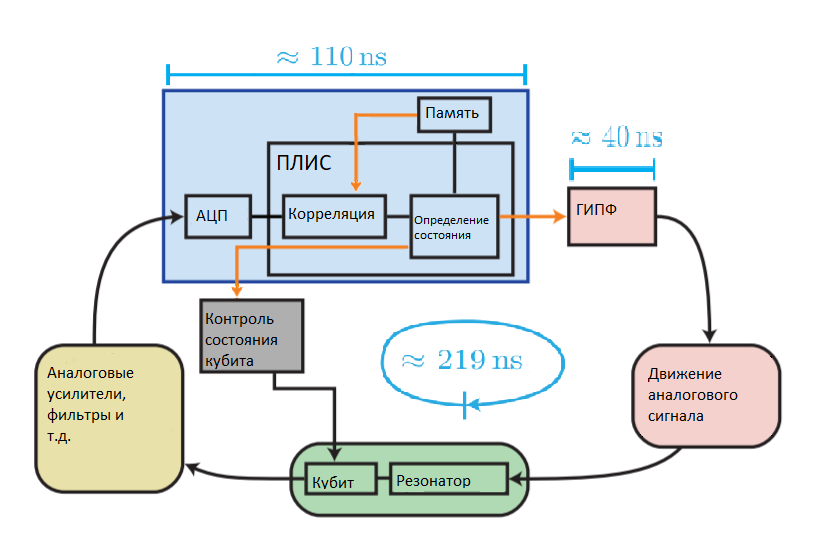
\includegraphics[width=0.7\linewidth]{pictures/feedback}
	\caption{Схема обратной связи}
	\label{fig:feedback}
\end{figure}

С помощью генератора сигналов произвольной формы на образец подаётся считывающий импульс, на выходе из образца он попадает в АЦП. По интерфейсу JESD204b он попадет в модуль ответственный за захват данных. Дополнительно в этот модуль был установлен линейный дискриминатор, подобный тому, что описан в (\ref{discr}). Этот дискриминатор считывает заранее записанные эталонные значения напряжения, соответствующие состояния $|0\rangle$ и $|1\rangle$, считает значение разности коэффициентов ковариации и в зависимости от величины этого значения принимает решение послать или не послать дополнительный сигнал на кубит. 

Как видно из схемы, на весь цикл уходит время порядка 200 нс, что существенно меньше времени релаксации. Использование быстрой обратной связи может быть использовано и в ряде других задач, таких как например передача классического ключа в алгоритме квантовой телепортации, выборочный контроль состояний одних кубитов, в зависимости от состояний других и т.д.



